\chapter{Comparison Between the MENP Framework and Traditional Hypotheses Testing Framework}
Chapter 4 showed that the MENP framework can be applied to spectrum sensing to achieve the largest probability of detection under any possible probability of false alarm constraints. This chapter presents a comparison between the MNEP framework and traditional hypotheses testing framework when applied to energy detection in the presence of two primary users. Two situations, one assuming the detector has no side information of primary users (for a given time slot, the detector does not know which primary signal could occupy the channel) and the other assuming the detector has perfect side information of primary users (for a given time slot, the detector knows which primary user could occupy the channel), are considered.  
Performance analysis results, which illustrate the performance for both frameworks, are presented.

\section{Energy Detection Without Side Information}
\subsection{System Model}
We consider a cognitive radio system where the licensed frequency spectrum could be occupied by one of two distinct signals $\{s_A, s_B\}$ or it could be vacant. 
Let $H_0$ denote the hypothesis under which the channel is free, $H_1$ denote the hypothesis under which the channel is occupied by $s_A$ or $s_B$.
Under hypothesis $H_1$, the channel is occupied by signal $s_A$ with probability $q$ and by signal $s_B$ with probability $1-q$, i.e. $Pr(s_A|H_1) = q$ and  $Pr(s_B|H_1) = 1-q$. Here $q$ is an unknown parameter for the detector. 
We are interested to test $H_0$ against $\bar{H}_0$. The block diagram of the system is illustrated in Figure \ref{pic: ch5 diagram}.  

\begin{figure}[!hbp]
\centering
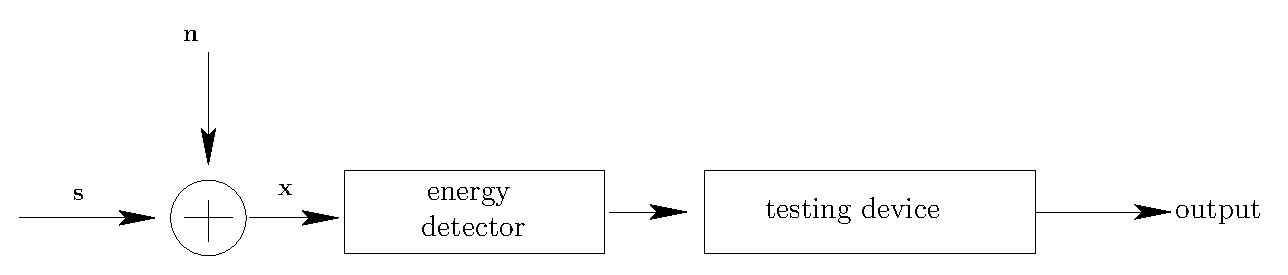
\includegraphics[width = \textwidth]{5/fig4.eps}
\caption{Block Diagram for Energy Detection}
\label{pic: ch5 diagram}
\end{figure}

The detector consists of a measuring device followed by a testing device. The measuring device observes the received signals and forms its energy using its sampled version. With this energy, the testing device employs a proper hypothesis testing framework to decide about the state of the channel. We assume during the detection, the channel status does not change. The input of the measuring device can be modeled as 
\begin{eqnarray}
  \mathbf{x} = \begin{cases}
    &\mathbf{n}\;\;\;\;\;\;\text{when $H_0$ is true}\\
    &\mathbf{n} + V\mathbf{s}_A + (1-V)\mathbf{s}_B\;\;\;\;\;\;\text{when $H_1$ is true}
  \end{cases}
  \label{equ:input2energy}
\end{eqnarray}
where
\begin{equation}
  \begin{cases}
	&\mathbf{x} = (x_0, x_1, \cdots, x_{N-1})\\
	&\mathbf{s}_A = (s_{A0}, s_{A1}, \cdots, s_{A(N-1)})\\
	&\mathbf{s}_B = (s_{B0}, s_{B1}, \cdots, s_{B(N-1)})\\
	&\mathbf{n} = (n_{0}, n_{1}, \cdots, n_{N-1})\,,
  \end{cases}
  \label{150621a1}
\end{equation}
and 
\begin{equation}
  V = \begin{cases}
    &0\;\;\;\;\;\;\text{with probability $q$}\\
    &1\;\;\;\;\;\;\text{with probability $1-q$}\,.
  \end{cases}
  \label{150621a2}
\end{equation}

Just like in section 4.1, 
we assume  $s_{Ai}$ $s_{Bi}$ and $n_i$ are zero-mean independent and identically distributed (iid) circularly symmetric complex Gaussian (CSCG) random variables with variances $2\sigma_{s_A}^2$, $2\sigma_{s_B}^2$ and $2\sigma_{n}^2$, i.e., $s_{Ai} \sim \mathcal{CN}(0, 2\sigma_{s_A}^2)$, $s_{Bi} \sim \mathcal{CN}(0, 2\sigma_{s_B}^2)$ and $n_i \sim \mathcal{CN}(0, 2\sigma_{n}^2)$.
Each sample $x_i = s_i + n_i$ ($s_i = s_{Ai}$ when $s_A$ is transmitting; $s_i = s_{Bi}$ when $s_B$ is transmitting) is governed by a probability law under each hypothesis. In our model
since the noise and signal are independent, $s_i+ n_i \sim \mathcal{CN}(0, 2(\sigma_{s}^2 + \sigma_n^2))$.  Define $\sigma_0^2 = \sigma_n^2$, $\sigma_1^2 = \sigma_{s_A}^2 + \sigma_n^2$ and $\sigma_2^2 = \sigma_{s_B}^2 + \sigma_n^2$, we can see
\begin{equation}
  \label{1129a1}
  \begin{split}
  n_i &\sim \mathcal{CN}(0, 2\sigma_0^2)\\
  n_i + s_{Ai} &\sim \mathcal{CN}(0, 2\sigma_1^2)\\
   n_i + s_{Bi}&\sim \mathcal{CN}(0, 2\sigma_2^2) \,,
  \end{split}
\end{equation}
thus we have 
\begin{equation}
   \begin{split}
     &\begin{pmatrix} x_{i_R} \\ x_{i_I} \end{pmatrix} \sim \mathcal{N}\Big( \begin{bmatrix} 0 \\ 0 \end{bmatrix}, \begin{bmatrix} \sigma_0^2 & 0\\ 0 & \sigma_0^2 \end{bmatrix} \Big) \text{when channel is free}\\
     &\begin{pmatrix} x_{i_R} \\ x_{i_I} \end{pmatrix} \sim \mathcal{N}\Big( \begin{bmatrix} 0 \\ 0 \end{bmatrix}, \begin{bmatrix} \sigma_1^2 & 0\\ 0 & \sigma_1^2 \end{bmatrix} \Big) \text{when channel is occupied by $s_A$}\\
     &\begin{pmatrix} x_{i_R} \\ x_{i_I} \end{pmatrix} \sim \mathcal{N}\Big( \begin{bmatrix} 0 \\ 0 \end{bmatrix}, \begin{bmatrix} \sigma_2^2 & 0\\ 0 & \sigma_2^2 \end{bmatrix} \Big) \text{when channel is occupied by $s_B$}
\end{split}
  \label{equ:xdistribution2}
\end{equation}
where $x_{i_R}$ and $x_{i_I}$ are real and imaginary components of $x_i$. 
Without losing generality, here we assume $\sigma_A^2 < \sigma_B^2$, so we have $\sigma_1^2 < \sigma_2^2$. 
Like in section 4.1, the output of measuring device is
\begin{equation} 
  Y = \sum_{i=0}^{N-1}|x_i|^2 = \sum_{i=0}^{N-1}(x_{i_R}^2+x_{i_I}^2)\,.
  \label{equ: testing device2}
\end{equation}
By observing $y$, a realization of $Y$, the testing device determines the status of the channel. From the analysis in section 3.3 and section 4.1, we know when the channel is free, $\frac{Y}{\sigma_0^2} \sim \chi^2(2N)$; when the channel is occupied by signal $s_A$, $\frac{Y}{\sigma_1^2} \sim \chi^2(2N)$; and when the channel is occupied by signal $s_B$, $\frac{Y}{\sigma_2^2} \sim \chi^2(2N)$.  The PDFs and CDFs under each situation are derived in section 3.3 and given as following: 
\def \CHISQUY[#1]{\frac{1}{#1 2^N\Gamma(N)}\left(\frac{y}{#1}\right)^{N-1}\exp\left(-\frac{y}{2#1}\right)}
\begin{equation}
  \begin{split}
   &f(y|H_0) = \CHISQUY[\sigma_0^2]\\
  &f(y|H_1, s_A)=  \CHISQUY[\sigma_1^2]\\
  &f(y|H_1, s_B)=  \CHISQUY[\sigma_2^2]\,;
\end{split}
  \label{20150621a4}
\end{equation} 
and
\begin{equation}
  \begin{split}
    F(y|H_0) &= F_{\chi^2(2N)}(\frac{y}{\sigma_0^2})\\
    F(y|H_1, s_A) &= F_{\chi^2(2N)}(\frac{y}{\sigma_1^2})\\
    F(y|H_1, s_B) &= F_{\chi^2(2N)}(\frac{y}{\sigma_2^2})\,,
  \end{split}
\end{equation}
where $F_{\chi^2(2N)}$ is the CDF of Chi-Square distribution with $2N$ degrees of freedom. 
For easy presentation, let $f_0(y) = f(y|H_0)$, $f_1(y|s_A) = f(y|H_1, s_A)$, $f_1(y|s_B) = f(y|H_1, s_B)$, $F_0(y) = F(y|H_0)$, $F_1(y|s_A) = F(y|H_1, s_A)$ and $F_1(y|s_B) = F(y|H_1, s_B)$. 
Since $\sigma_0^2 < \sigma_1^2 < \sigma_2^2$, we have 
\begin{equation}
  \frac{y}{\sigma_0^2} \geq \frac{y}{\sigma_1^2} \geq \frac{y}{\sigma_2^2}
\end{equation}
and since the CDF is monotonically non-decreasing, we have 
\begin{equation}
  F_{\chi^2(2N)}(\frac{y}{\sigma_0^2}) \geq F_{\chi^2(2N)}(\frac{y}{\sigma_1^2}) \geq  F_{\chi^2(2N)}(\frac{y}{\sigma_2^2})
  \label{20150701a0}
\end{equation}
\begin{equation} 
\therefore  F_0(y) \geq F_1(y|s_A) \geq F_1(y|s_B)
  \label{20150623a1}
\end{equation}
with equality when $y \rightarrow +\infty$.

From above discussion, it can be seen under hypothesis $H_1$ the PDF of $Y$ can be written as
\begin{equation}
  \begin{split}
    f_1(y) &= f_1(y|s_A)\text{Pr}(s_A|H_1) + f_1(y|s_B)\text{Pr}(s_B|H_1)\\
         &= f_1(y|s_A)q + f_1(y|s_B)(1-q)\,,
\end{split}
  \label{20150621a7}
\end{equation}
and thus we have
\begin{equation}
  \begin{split}
    H_0:\;\;\;\;\;&f_0(y) = \CHISQUY[\sigma_0^2]\\
    H_1:\;\;\;\;\;&f_1(y) = q\CHISQUY[\sigma_1^2] + (1-q)\CHISQUY[\sigma_2^2]\,.
  \end{split}
  \label{20150621a81}
\end{equation}

As we can see, $H_0$ is a simple hypothesis and $H_1$ is a composite hypothesis with unknown parameter $q \in [0, 1]$. 
The LR test for problem  \eqref{20150621a81} is
\begin{equation}
  \frac{f_1(y)}{f_0(y)} \substack{H_1 \\ \geq \\ < \\ H_0} \tau\,.
\end{equation}
Substitute $f_0(y)$ and $f_1(y)$ into above equation, we have 
\begin{equation}
  q\left(\frac{\sigma_0^2}{\sigma_1^2}\right)^N\exp\left( (\frac{1}{2\sigma_0^2} -  \frac{1}{2\sigma_1^2}  )y \right)
+ (1-q) \left(\frac{\sigma_0^2}{\sigma_2^2}\right)^N\exp\left( (\frac{1}{2\sigma_0^2} -  \frac{1}{2\sigma_2^2}  )y \right)
\substack{H_1 \\ \geq \\ < \\ H_0} \tau\,.
\label{20150622a0}
\end{equation}
For a specific $q$, define 
\begin{equation}
  g_q(y) = q\left(\frac{\sigma_0^2}{\sigma_1^2}\right)^N\exp\left( (\frac{1}{2\sigma_0^2} -  \frac{1}{2\sigma_1^2}  )y \right)
+ (1-q) \left(\frac{\sigma_0^2}{\sigma_2^2}\right)^N\exp\left( (\frac{1}{2\sigma_0^2} -  \frac{1}{2\sigma_2^2}  )y \right)\,
\end{equation}
and \eqref{20150622a0} can be written as
\begin{equation}
  g_q(y) \substack{H_1 \\ \geq \\ < \\ H_0} \tau\,.
  \label{20150622a1}
\end{equation}
Since $q, 1-q \geq 0$ and $(\frac{1}{2\sigma_0^2} -  \frac{1}{2\sigma_1^2}  ), (\frac{1}{2\sigma_0^2} -  \frac{1}{2\sigma_2^2}  ) >  0$, we know $g_q(y)$ is a monotonic increasing function and $g^{-1}_q(y) $ exists.  
Let $V_\tau = g^{-1}_q(\tau)$, since $g(y)$ is a monotonic increasing function, we have 
\begin{equation}
  \begin{cases}
    &y > V_\tau\;\;\;\;g(y)_q > \tau\\
    &y < V_\tau\;\;\;\;g(y)_q < \tau\,.
  \end{cases}
\end{equation}
Hence \eqref{20150622a1} can be written in form of 
\begin{equation}
  y  \substack{H_1 \\ \geq \\ < \\ H_0} V_\tau\,.
  \label{20150622a2}
\end{equation}

By using decision rule \eqref{20150622a2}, the probability of detection and the probability of false alarm can be written in form of 
\begin{equation}
  P_d = \int_{0}^{V_\tau} f_0(y) \mathrm{d}y = F_0(V_\tau)
  \label{20150701a3}
\end{equation}
\begin{equation}
  \begin{split}
  P_{f,q} &= \int_{0}^{V_\tau} (qf_1(y|s_A) + (1-q)f_1(y|s_B))\mathrm{d}y\\
  &= q\int_{0}^{V_\tau} f_1(y|s_A)\mathrm{d}y  + (1-q)\int_0^{V_\tau}f_1(y|s_B)\mathrm{d}y\\
      &= qF_1(V_\tau|s_A) + (1-q)F_1(V_\tau|s_B)\,.
    \end{split}
    \label{20150622a3}
  \end{equation}
  Here we use $P_{f,q}$ to present the probability of false alarm for a specific $q$.
  As we can see from \eqref{20150622a3},  $P_{f,q}$ depends on both $V_\tau$ and $q$.  
  First assume the detector knows $q$, in such situations \eqref{20150622a2} is a Neyman Pearson decision rule and  we can adjust the value of $V_\tau$ to construct a NP test with $P_{f,q} = c$.
  For example, let $q = 1$ and $V_\tau$ is chosen such that $F_1(V_\tau|s_A) = c$, i.e. $V_\tau = F_1^{-1}(c|s_A)$. From \eqref{20150622a3} we have 
\begin{equation}
  P_{f,1} = F_1(V_\tau|s_A) = c\,.
  \label{20150623a0}
\end{equation}
Thus it can be concluded that when $q = 1$ decision rule 
\begin{equation}
\delta^\ast \;\;\;\;y \substack{H_1 \\ \geq \\ < \\ H_0} V_\tau\;\;\;\;\;\;\text{where $V_\tau = F_1^{-1}(c|s_A)$}
\label{20150705a0}
\end{equation}
is NP decision rule with  $P_{f, 1} = c$. Let $\delta$ be any other decision rule such that $P_{f, 1}(\delta) \leq c$ is satisfied, from the property of NP test, it can be concluded that $P_d(\delta^\ast) \geq P_d(\delta)$.  

In practice the value of $q$ is unknown for the detector. In such case, we will show $ \delta^\ast$ given in \eqref{20150705a0} is the uniformly most powerful (UMP) test of size $c$ ($c \in (0, 1)$). 
 
 The \textbf{uniformly most powerful (UMP) test} of size $c$ is defined as following \cite{LehmannTest, poor1994introduction, casella2002statistical}:
\textit{
  Let $f(x|H_0, \theta_0)$ $f(x|H_1, \theta_1)$ be PDFs under hypotheses $H_0$ and $H_1$. $\theta_0, \theta_1$ are unknown deterministic parameter and $\theta_0 \in \Theta_0, \theta_1 \in \Theta_1$. A UMP test is a test that maximizes $P_{d, \theta_0}$ for every  $\theta_0 \in \Theta_0$ subject to the constraint $(P_{f,\theta_1} \leq c\;\;\;\;\forall \theta_1 \in \Theta_1)$, i.e. }
\begin{equation}
  \begin{split}
    \max\;\;\;\;&P_{d, \theta_0}\;\;\;\theta_0 \in \Theta_0\\
    \text{s.t.}\;\;\;\;&P_{f, \theta_1} \leq c\;\;\;\theta_1 \in \Theta_1
  \end{split}
\end{equation}

Thus we can see,  $\delta$ of \eqref{20150623a0}  is a UMP decision rule if: 
  \\(1) $\forall \theta_1 \in \Theta_1$, we have $P_{f, \theta_1}(\delta) \leq c$;
  \\(2) Let $\delta'$ be a decision rule satisfying (1), then  $\forall \theta_0 \in \Theta_0$, we have $P_{d,\theta_0}(\delta) \geq P_{d, \theta_0}(\delta')$. 

  In our case, $H_1$ is a composite hypothesis with unknown parameter $q \in [0, 1]$ and $H_0$ is a simple hypothesis. From the definition of the UMP test,  we can see $\delta^\ast$ of \eqref{20150705a0} is a UMP test of size $c$ if:
\\(a) for any $q \in [0, 1]$, we have $P_{f,q}(\delta^\ast) \leq c$;
\\(b) Assume $\delta'$ is a decision rule satisfying condition (a), we have $P_d(\delta^\ast) \geq P_d(\delta')$.  

First, we will show decision rule $\delta^\ast$ satisfies condition (a). From \eqref{20150623a1}, \eqref{20150622a3} and \eqref{20150623a0}, we have 
\begin{equation}
  \begin{split}
    P_{f,q}(\delta^\ast) &= qF_1(V_\tau|s_A) + (1-q)F_1(V_\tau|s_B)\\
    &\leq qF_1(V_\tau|s_A) + (1-q)F_1(V_\tau|s_A)\\
    &= F_1(V_\tau|s_A) = c\,.
  \end{split}
\end{equation}
\begin{equation}
  \therefore P_{f,q}(\delta^\ast) \leq c
  \label{20150705a1}
\end{equation}
Thus we can see by using decision rule $\delta^\ast$ of \eqref{20150623a0}, for all $q \in [0, 1]$, $P_{f,q}(\delta^\ast) \leq c$ is satisfied.

Next we will show for any decision rule $\delta'$ satisfying condition (a), we have $P_d(\delta^\ast) \geq P_d(\delta')$.  
Assume $\delta'$ is a decision rule satisfying condition (a), then we have  $P_{f,1}(\delta') \leq c$.
Since $\delta^\ast$ is NP optimal for $q=1$, then $P_d(\delta^\ast)\geq P_d(\delta')$ for $q =1$.
For any $q \in [0, 1]$, we have $P_{f_q} \leq c$ because of the definition of the test $\delta'$. Since $P_d(\delta^\ast)$ and $P_d(\delta')$ do not depend on $q$, we have $P_d(\delta^\ast) \geq P_d(\delta')$ for all $q \in [0, 1]$.
Hence decision rule $\delta^\ast$ also satisfies condition (b). Since decision rule $\delta^\ast$ satisfies both condition (a) and (b), it is the UMP test of size $c$.    


%\subsection{A Comparison Between the MENP Test and the UMP Test for Energy Detector with no Side Information}
%A comparison between the MENP test and the UMP test for energy detection without side information is summarized in Table 5.1.

%\begin{table}[]
%\centering
%\label{my-label}
%\resizebox{\textwidth}{!}{%
%\begin{tabular}{|l|l|l|}
%\hline
%                                                                 & MENP Test                                                                                                                                                                  & UMP Test                                                                                                                                                                 \\ \hline
%\begin{tabular}[c]{@{}l@{}}Hypotheses\\ Description\end{tabular} & \begin{tabular}[c]{@{}l@{}}$H_0:$   The channel is ideal;\\ $H_1:$   The channel is occupied by $s_A$;\\ $H_2:$   The channel is occupied by $s_B$.\end{tabular}           & \begin{tabular}[c]{@{}l@{}}$H_0:$  The channel is ideal;\\ $H_1:$  The channel is occupied by $s_A$ or $s_B$.\end{tabular}                                               \\ \hline
%Object                                                           & \begin{tabular}[c]{@{}l@{}}A MENP decision rule achieve the largest \\ $P_d$ among all decision rules satisfying \\ $P_{f_1} \leq c_1$ and $P_{f_2} \leq c_2$\end{tabular} & \begin{tabular}[c]{@{}l@{}}A UMP decision rule achieve the largest \\ $P_d$  among all decision rules satisfying \\ $\forall q \in [0, 1]$ $P_{f,q} \leq c$\end{tabular} \\ \hline
%\begin{tabular}[c]{@{}l@{}}Decision \\ Rule\end{tabular}         & $y \substack{ H_0 \\ \leq \\ > \\ \bar{H}_0} V_{\tau, MENP}$                                                                                                                & $y \substack{H_0 \\ \leq \\ > \\ \bar{H}_0} V_{\tau, UMP}$                                                                                                               \\ \hline
%$V_\tau$                                                         & $\min \{F_1^{-1}(c_1 | s_A), F_1^{-1}(c_2 | s_B) \}$                                                                                                                       & $F_1^{-1}(c | s_A)$                                                                                                                                                      \\ \hline
%$P_d$                                                            & $F_0(V_{\tau, MENP})$                                                                                                                                                      & $F_0(V_{\tau, UMP})$                                                                                                                                                     \\ \hline
%$P_f$                                                            & $P_{f_1} = F_1(V_{\tau, MENP} | s_A), P_{f_2} = F_1(V_{\tau, MENP} | s_B)$                                                                                                                 & $P_{f,q} = q F_1(V_{\tau, UMP} | s_A) + (1-q) F_1(V_{\tau, UMP} | s_B)$                                                                                                                \\ \hline
%\end{tabular}
%}
%\caption{A comparison between MENP test and UMP test when applying to energy detection}
%\end{table}

%From Table 5.1 we can see the MENP test are designed to provide different protection to different primary users while the UMP test 
%As we can see, for both MENP test and UMP test the decision rule has the same form, but the values of threshold ($V_{\tau, MENP}$, $V_{\tau, UMP}$) are different.  If $V_{\tau, MENP} \geq V_{\tau, UMP}$, the probability of detection achieved by MNEP is larger than that of the UMP test, vice versa. 




\subsection{Performance Comparison}
In this section, we compare the performance of the UMP test with the performance of the MENP test when the detector has no side information.
Similar to section 4.1.2, we set $\sigma_n^2= 0.1$, $\sigma_{s_A}^2 = 0.05$ $\sigma_{s_B}^2 = 0.15$ and $N=20$, leading to  $\sigma_0^2 = 0.1$, $\sigma_1^2=0.15$ and $\sigma_2^2 = 0.25$. 
First we consider the performance of the UMP test. 
We let $c$ increase from $0$ to $0.2$ in steps of $10^{-6}$. For each value of $c$, we use $V_\tau = F_1^{-1}(c|s_A)$ to compute the corresponding threshold $V_\tau$. By substituting $V_\tau$ into \eqref{20150701a3} we can get the associated $P_d$. The performance of the UMP test is illustrated in Figure \ref{pic:20150701a0}. 
The performance of energy detection using MENP framework is also shown in Figure \ref{pic:20150701a0}. Under MENP framework, $P_d$ is related to both $c_1$ and $c_2$. In Figure \ref{pic:20150701a0}, we plot the relationship between $P_d$ and $c_1$ when $c_2$ is fixed (In this case we set $c_1 = c$). Then we illustrate the relationship between $P_d$ and $c_2$ when $c_1$ is fixed (In this case we set $c_2 = c$).   

\begin{figure}[!hbp]
\centering
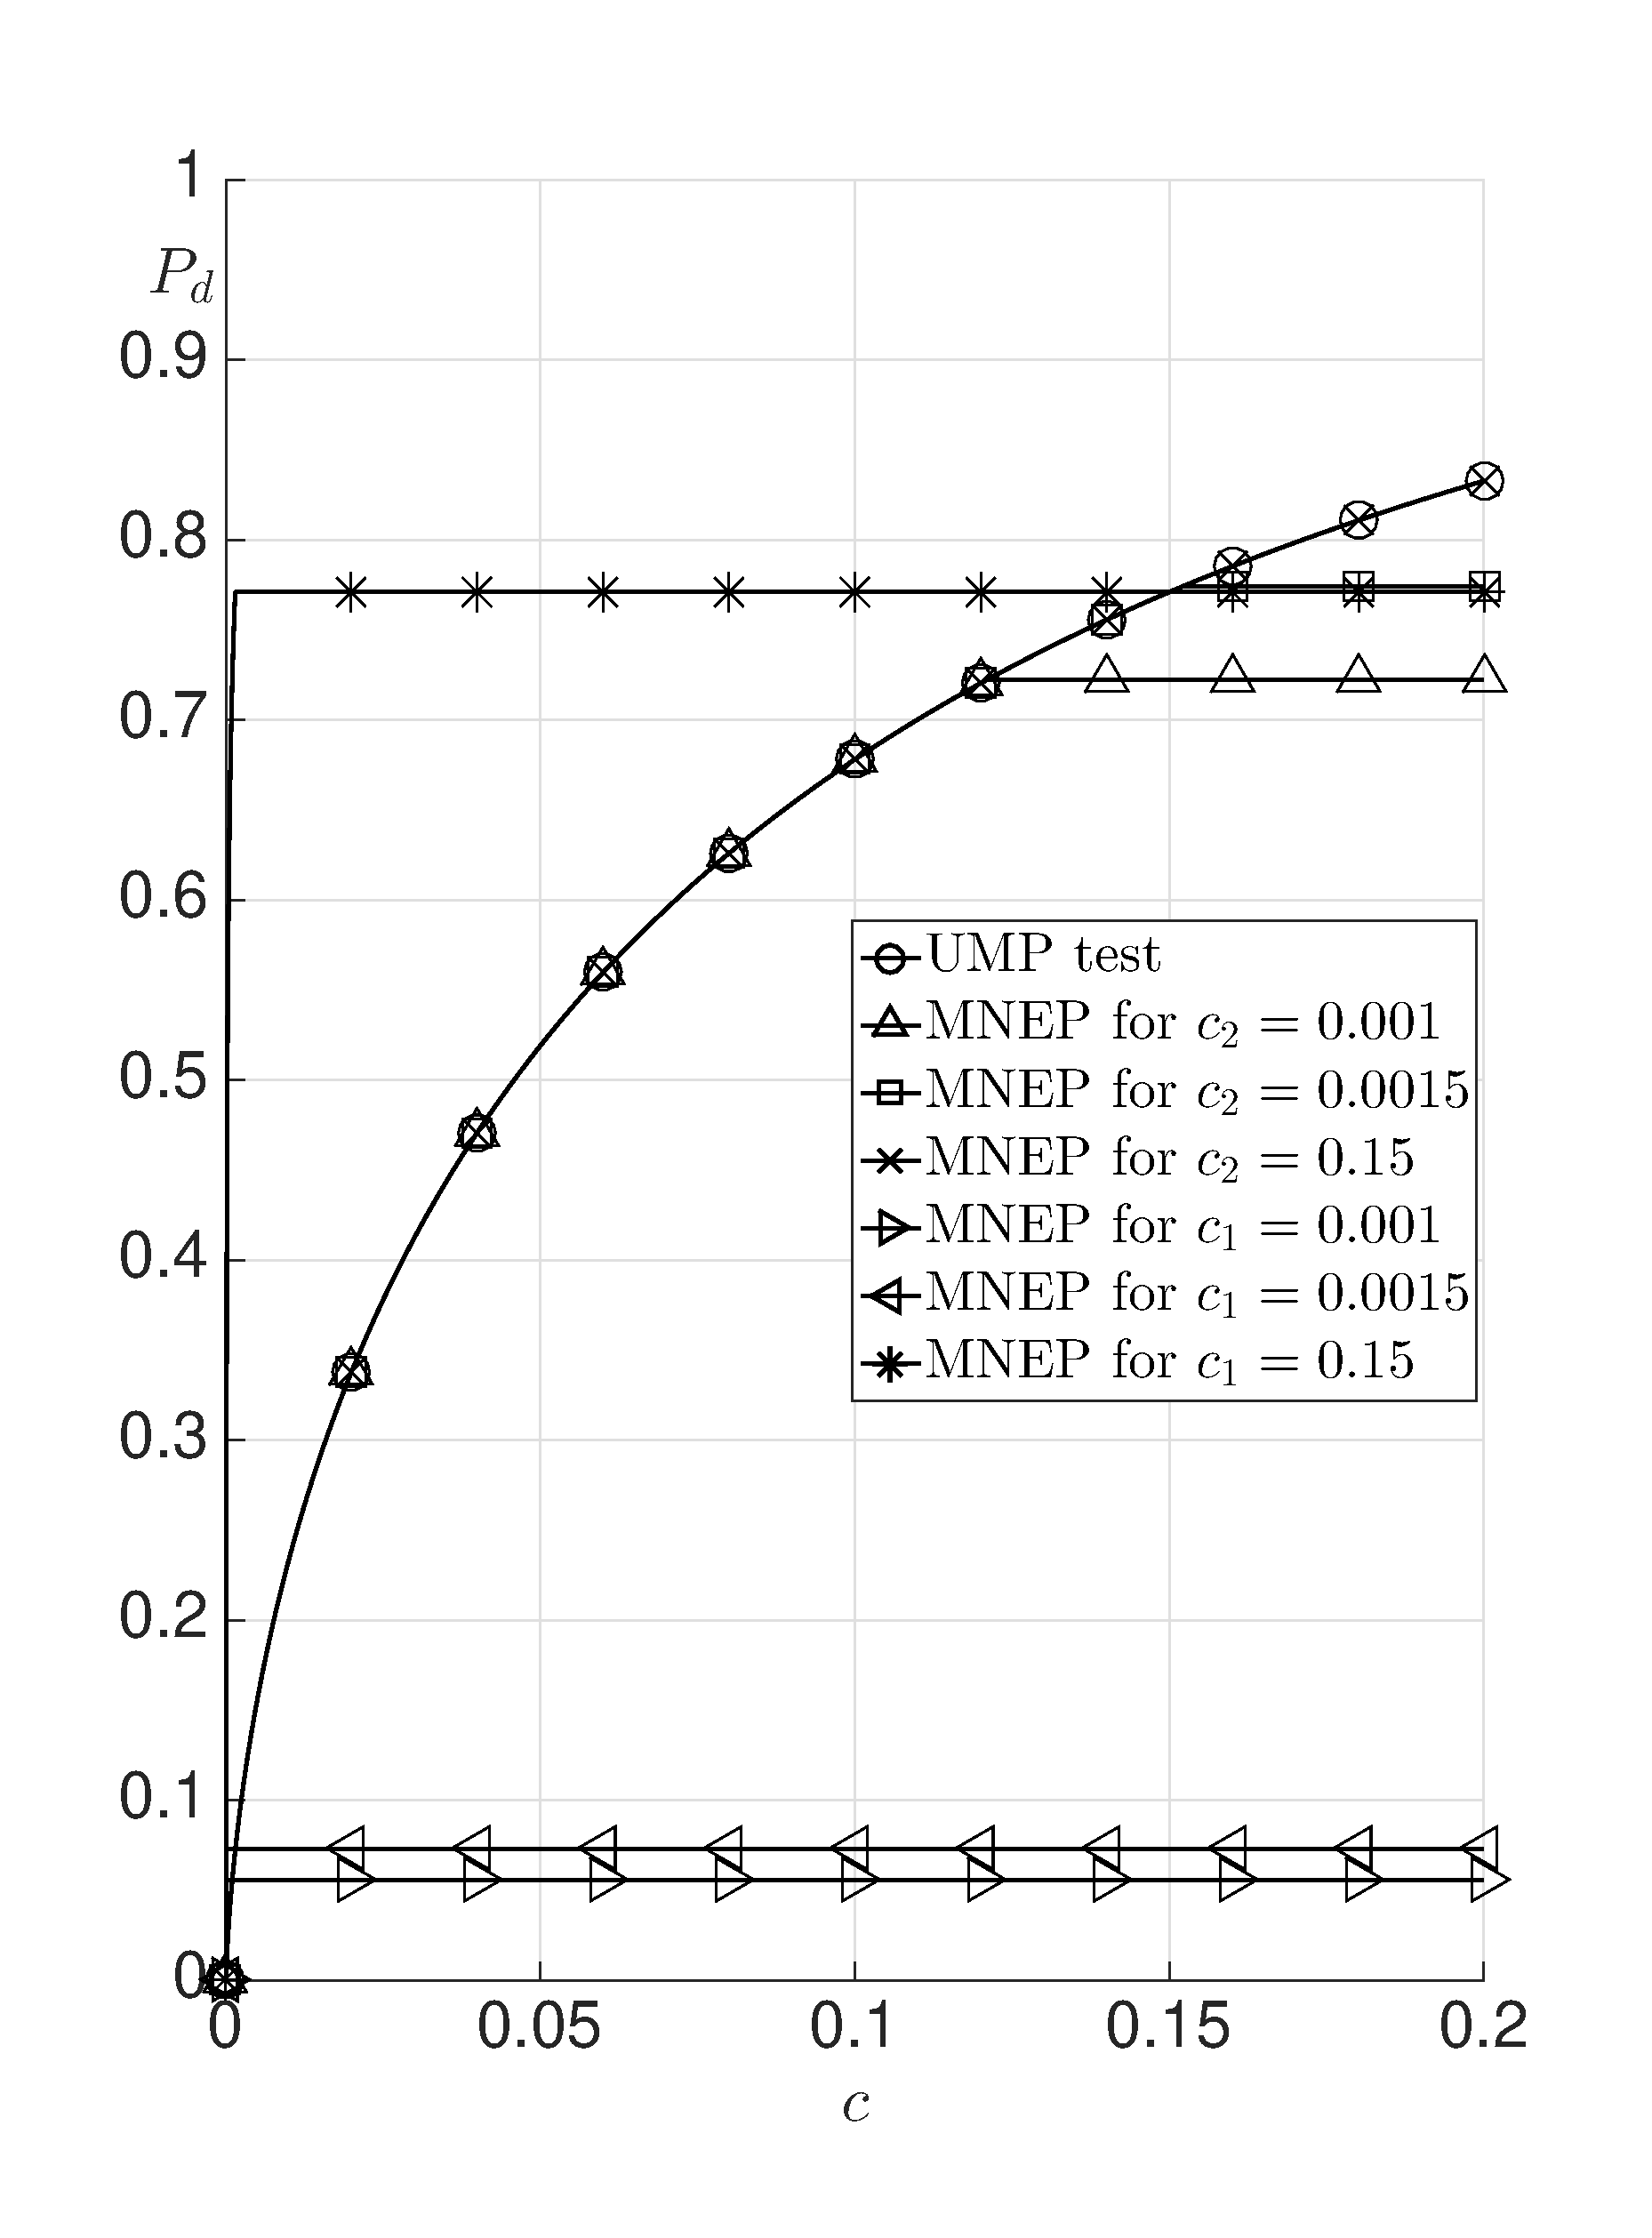
\includegraphics[width = 14cm]{5/noSI.eps}
\caption{A comparison between the UMP test and MENP test}
\label{pic:20150701a0}
\end{figure}

As we can observe, when $c_1$ is fixed to $0.15$ and $c_2$ smaller than $0.15$, the performance of MENP test is better than the UMP test. This is not contradictory with the definition of the UMP test. As we have discussed in section 5.1.1, a UMP decision rule is a decision rule such that among all decision rules satisfying $\forall q \in [0, 1]$ $P_{f,q} \leq c$, it maximizes $P_d$. With the MENP test, for $\forall q \in [0, 1]$ we cannot necessarily have $P_{f,q} \leq c$, hence it is possible that the $P_d$ for the MENP test is larger than the $P_d$ for the UMP test.  For example, when $c_2 = c = 0.05$ and $c_1 = 0.15$, with the UMP test we have $P_d = 0.5192$; with the MENP test we have $P_d = 0.7711$. However by using this MENP test, when $q = 1$ we have $P_f = 0.15 > c = 0.05$, i.e. $P_{f,1} > c$.   

Furthermore, for both the MENP and the UMP tests, the decision rule can be written in form of
\begin{equation}
  y \substack{\bar{H}_0\\ \geq\\ < \\ H_0 } V_\tau\,,
  \label{20150701a4}
\end{equation}
and the probability of detection is 
\begin{equation}
  P_d = F_0(V_\tau)\,.
  \label{20150701a5}
\end{equation}

In the MENP test, $V_\tau$ is determined by $V_{\tau MENP}= \min (F_1^{-1}(c_1|s_A), F_1^{-1}(c_2|s_B))$; in the UMP test, $V_\tau$ is determined by $V_{\tau UMP} = F_1^{-1}(c|s_A)$. When $V_{\tau MENP}  \geq V_{\tau UMP}$, then the $P_d$ achieved by the MENP test is no smaller than that achieved by UMP test. When $V_{\tau MENP}  \leq V_{\tau UMP}$, then the $P_d$ achieved by MENP test is no larger than that achieved by UMP test. 
With the MENP test, when $c_2$ is fixed and $c_1 = c$, we have $\min (F_1^{-1}(c_1|s_A), F_1^{-1}(c_2|s_B)) \leq F_1^{-1}(c_1|s_A) = F_1^{-1}(c|s_A) $, i.e. 
$V_{\tau MENP} \leq V_{\tau UMP}$.
Hence we can conclude that when $c_2$ is fixed and $c_1 = c$, the $P_d$ achieved by MENP test is no larger than that achieved by UMP test. When $F_1^{-1}(c_1|s_A) \geq F_2^{-1}(c_2|s_B)$, i.e. $\min (F_1^{-1}(c_1|s_A), F_1^{-1}(c_2|s_B)) = F_1^{-1}(c_1|s_A) = F_1^{-1}(c|s_A) $, the equality holds.  For example when $c_2 $ is fixed to $0.15$, when $c_1 = c \in [0, 0.2]$, we have $F_1^{-1}(c_1|s_A) \geq F_2^{-1}(c_2|s_B)$ and the performance of the MENP test and the UMP test are equal. 
Above conclusions can be verified in Figure \ref{pic:20150701a0}. 

Finally, we consider the performance of the MENP test when $c_1$ is fixed to $0.15$. As we observe in this case when $c_2$ is smaller than $0.15$ the performance of MENP test is better than the UMP test. This is because when $c_2 = c  \leq 0.15$, $\min (F_1^{-1}(0.15|s_A), F_1^{-1}(c_2|s_B)) > F_1^{-1}(c|s_A)$, i.e. $V_{\tau MENP} \geq V_{\tau UMP }$.   Hence the $P_d$ achieved by MENP test is larger than that achieved by UMP test. 


From above discussion we can conclude that with $c_2$ fixed and $c_1 = c$, the UMP outperforms the MENP test, however when $F_1^{-1}(c_1|s_A) \geq F_2^{-1}(c_2|s_B)$, the performance of MENP test and UMP test are the same. With $c_1$ fixed and $c_2  = c$, it is possible that the MENP test outperforms the UMP test. This is because the UMP test maximizes $P_d$ among all decision rules satisfying $\forall q \in [0, 1] $ $P_{f,q} \leq c$, but 
in the MENP test $P_d$ is associated with two parameters $c_1, c_2$.  As we have shown in section 3.3, when $c_1$ (or $c_2$) increases and $c_2$ (or $c_1$) remains the same, $P_d$ will either remain the same or increases. When we set $c_2 = c$ and $c_1$ is large enough, it is possible that the $P_d$ achieved by the MENP test is larger than the $P_d$ achieved by the UMP test.
\typeout{}
\section{Energy Detection with Perfect Side Information}
\subsection{System Model}
We consider a cognitive radio system where the licensed frequency spectrum could be occupied by one of two distinct signals $\{s_A, s_B\}$ or it could be vacant. 
Assume the detector has perfect side information of primary users, i.e. for a specific time slot the detector knows which primary user could occupy the channel. For easy presentation, let $T_A$ presents the time slot during which the channel can be either free or occupied by primary signal $s_A$. Let $T_B$ denote the time slot during which the channel can be either free or occupied by primary signal $s_B$. We can see, during time slot $T_A$, primary user $s_B$ will not present in the channel and during time slot $T_B$ primary user $s_A$ will not present in the channel. Since the detector has perfect side information, it knows the beginnings and endings for $T_A$ and $T_B$. Let $H_0$ denote the hypothesis under which the channel is free,  $H_1$ denote the hypothesis under which the channel is occupied by $s_A$ and $H_2$ denote the hypothesis under which the channel is occupied by $s_B$, i.e.
\begin{equation}
\begin{cases}
H_0:\;\;\;\;\text{channel is free}\\
H_1:\;\;\;\;\text{channel is occupied by $s_A$}\\
H_2:\;\;\;\;\text{channel is occupied by $s_B$}\,.
\end{cases}
\end{equation} 

During time slot $T_A$, we  test $H_0$ against $H_1$; during time slot $T_B$, we test $H_0$ against $H_2$. 
Even though there are three hypotheses, for a specific time slot, it is still a two hypotheses testing problem.  
For both $T_A$ and $T_B$, we use an energy detector to decide the status of the channel. Let $\mathbf{x}$ denote the input of the detector, $Y$ denote the testing statistics of the received signal (in this case, $Y$ is the energy of the sampled signal), $n$  denote the system noise and $s_A$ or $s_B$ denotes the transmitted signal. Hence we have
\begin{eqnarray}
  \mathbf{x} = \begin{cases}
    &\mathbf{n}\;\;\;\;\;\;\text{when the channel is free}\\
    &\mathbf{n} + \mathbf{s}_A \;\;\;\;\;\;\text{when the channel is occupied by $s_A$}\\
    &\mathbf{n} + \mathbf{s}_B \;\;\;\;\;\;\text{when the channel is occupied by $s_B$}
  \end{cases}
  \label{20150627a0}
\end{eqnarray}
where
\begin{equation}
  \begin{cases}
  &\mathbf{x} = (x_0, x_1, \cdots, x_{N-1})\\
  &\mathbf{s}_A = (s_{A0}, s_{A1}, \cdots, s_{A(N-1)})\\
  &\mathbf{s}_B = (s_{B0}, s_{B1}, \cdots, s_{B(N-1)})\\
  &\mathbf{n} = (n_{0}, n_{1}, \cdots, n_{N-1})
  \end{cases}
  \label{20150627a1}
\end{equation}
and
\begin{equation}
Y = \sum_{i=0}^{N-1} x_i^2\,.
\end{equation}
As in section 4.1 and section 5.1, we assume  $s_{Ai}$ $s_{Bi}$ and $n_i$ are zero-mean independent and identically distributed (iid) circularly symmetric complex Gaussian (CSCG) random variables with variances $2\sigma_{s_A}^2$, $2\sigma_{s_B}^2$ and $2\sigma_{n}^2$, i.e., $s_{Ai} \sim \mathcal{CN}(0, 2\sigma_{s_A}^2)$, $s_{Bi} \sim \mathcal{CN}(0, 2\sigma_{s_B}^2)$ and $n_i \sim \mathcal{CN}(0, 2\sigma_{n}^2)$.
Each noisy sample $x_i = s_i + n_i$ is governed by a probability law under each hypothesis. In our model
since the noise and signal are independent, $s_i+ n_i \sim \mathcal{CN}(0, 2(\sigma_{s}^2 + \sigma_n^2))$.  Define $\sigma_0^2 = \sigma_n^2$, $\sigma_1^2 = \sigma_{s_A}^2 + \sigma_n^2$ and $\sigma_2^2 = \sigma_{s_B}^2 + \sigma_n^2$, we can see
\begin{equation}
  \label{20150627a2}
  \begin{split}
  n_i &\sim \mathcal{CN}(0, 2\sigma_0^2)\\
  n_i + s_{Ai} &\sim \mathcal{CN}(0, 2\sigma_1^2)\\
   n_i + s_{Bi}&\sim \mathcal{CN}(0, 2\sigma_2^2) \,.
  \end{split}
\end{equation}

In the following we consider the decision rule during time slot $T_A$. From the definition, we know during $T_A$ only primary signal $s_A$ could present in the channel and we are interested to test $H_0$ against $H_1$:
\begin{equation}
  \begin{split}
&H_0:\;\;\;\;\text{the channel is free}\\
&H_1:\;\;\;\;\text{the channel is occupied by $s_A$}\,.
\end{split}
\end{equation}

In section 4.1.1, we have proved 
\begin{equation}
\begin{split}
  H_0:\;\;\;\;&\frac{Y}{\sigma_0^2} \sim \chi^2(2N)\\
H_1:\;\;\;\;&\frac{Y}{\sigma_1^2} \sim \chi^2(2N)
\end{split}
\end{equation}
where $\chi^2(2N)$ is the Chi-square distribution with $2N$ degrees of freedom. Let $y$ be a realization of $Y$, in section 3.3, we have shown the PDFs of $y$ under hypotheses $H_0$ and $H_1$ are 
\begin{equation}
  \begin{split}
    H_0:\;\;\;\;\;&f_0(y) = \CHISQUY[\sigma_0^2]\\
    H_1:\;\;\;\;\;&f_{1}(y) = \CHISQUY[\sigma_1^2]\,.
  \end{split}
  \label{20150621a8}
\end{equation}

We use the Neyman Pearson decision rule to test $H_0$ against $H_1$, and hence the decision rule can be written as
\begin{equation}
  \frac{f_1(y)}{f_0(y)} \substack{\bar{H}_0 \\ \geq \\ < \\ H_0} \tau\,.
\end{equation}
Substituting \eqref{20150621a8} into above equation leads to 
\begin{equation}
  \frac{\CHISQUY[\sigma_1^2]}{\CHISQUY[\sigma_0^2]}\substack{\bar{H}_0 \\ \geq \\ < \\ H_0} \tau
\end{equation}
\begin{equation}
  \left(\frac{\sigma_0^2}{\sigma_1^2}\right)^N\exp\left( (\frac{1}{2\sigma_0^2} -  \frac{1}{2\sigma_1^2}  )y \right)\substack{\bar{H}_0 \\ \geq \\ < \\ H_0} \tau
\end{equation}
Defining 
\begin{equation}
  g(y) = \left(\frac{\sigma_0^2}{\sigma_1^2}\right)^N\exp\left( (\frac{1}{2\sigma_0^2} -  \frac{1}{2\sigma_1^2}  )y \right)
  \label{20150629a0}
\end{equation}
\eqref{20150629a0} can be written as
\begin{equation}
  g(y) \substack{\bar{H}_0 \\ \geq \\ < \\ H_0} \tau\,.
  \label{20150622a12}
\end{equation}
Since $(\frac{1}{2\sigma_0^2} -  \frac{1}{2\sigma_1^2}  ) >  0$, we know $g(y)$ is a monotonic increasing function and $g^{-1}(y) $ exists.  
Let $V_\tau = g^{-1}(\tau)$, since $g(y)$ is a monotonic increasing function, we have 
\begin{equation}
  \begin{cases}
    &y > V_\tau\;\;\;\;g(y) > \tau\\
    &y < V_\tau\;\;\;\;g(y) < \tau\,.
  \end{cases}
\end{equation}
Hence \eqref{20150622a12} can be written in the form 
\begin{equation}
  y  \substack{\bar{H}_0 \\ \geq \\ < \\ H_0} V_\tau\,.
  \label{20150622a22}
\end{equation}
By using decision rule \eqref{20150622a22}, the probability of detection and the probability of false alarm can be written in form of 
\begin{equation}
  \begin{split}
  P_d &= \int_{0}^{V_\tau} f_0(y) \mathrm{d}y = F_0(V_\tau)\\
  P_f &= \int_{0}^{V_\tau} f_1(y) \mathrm{d}y= F_1(V_\tau)\,.
    \end{split}
    \label{20150622a32}
  \end{equation}
  where $F_0$ is the CDF of $Y$ when the channel is free and $F_1$ is the CDF of $Y$ when the channel is occupied by primary signal $s_A$. For a given $c \in (0, 1)$, to achieve the largest  $P_d$ while keeping $P_f \leq c$, we should choose the threshold $V_\tau$ such that $F_1(V_\tau) = c$ is satisfied, i.e. $V_\tau = F^{-1}_1(c)$. 

Next we consider the decision rule during time slot $T_B$. From the definition, we know during $T_B$ only primary signal $s_B$ could present in the channel and we are interested to test $H_0$ against $H_2$:
\begin{equation}
  \begin{split}
&H_0:\;\;\;\;\text{the channel is free}\\
&H_2:\;\;\;\;\text{the channel is occupied by $s_B$}\,.
\end{split}
\end{equation}
In section 4.1.1, it has been proved 
\begin{equation}
\begin{split}
  H_0:\;\;\;\;&\frac{Y}{\sigma_0^2} \sim \chi^2(2N)\\
H_2:\;\;\;\;&\frac{Y}{\sigma_2^2} \sim \chi^2(2N)
\end{split}
\end{equation}
thus we have
\begin{equation}
  \begin{split}
    H_0:\;\;\;\;\;&f_0(y) = \CHISQUY[\sigma_0^2]\\
    H_2:\;\;\;\;\;&f_{2}(y) = \CHISQUY[\sigma_2^2]\,.
  \end{split}
\end{equation}

By using the same method as in deriving the Neyman Pearson decision rule for time slot $T_A$, we can get the Neyman Pearson decision rule for testing $H_0$ against $H_2$:
\begin{equation}
  y  \substack{\bar{H}_0 \\ \geq \\ < \\ H_0} V_\tau'\,,
  \label{20150628a0}
\end{equation}
and  
\begin{equation}
  \begin{split}
  P_d &= \int_{0}^{V_\tau'} f_0(y) \mathrm{d}y = F_0(V_\tau')\\
  P_f &= \int_{0}^{V_\tau'} f_2(y) \mathrm{d}y= F_2(V_\tau')\,.
    \end{split}
    \label{20150628a1}
  \end{equation}
For a given $c \in (0, 1)$, to achieve the largest  $P_d$ while keeping $P_f \leq c$, we should choose $V_\tau'$ such that $F_2(V_\tau') = c$ is satisfied, i.e. $V_\tau' = F^{-1}_2(c)$. 

From the above discussion, we can see when the detector has perfect side information of primary users, to achieve the largest $P_d$ while keeping $P_f \leq c$, the decision rule $\delta_{NP}$ can be written in form of:
\begin{equation}
  \delta_{NP}:\;\;
\begin{cases}
 y  \substack{\bar{H}_0 \\ \geq \\ < \\ H_0} V_\tau\;\;\;\;V_\tau = F_1^{-1}(c)\;\;\;\;\text{during time slot $T_A$}\\
y  \substack{\bar{H}_0 \\ \geq \\ < \\ H_0} V_\tau'\;\;\;\;V_\tau' = F_2^{-1}(c)\;\;\;\;\text{during time slot $T_B$}\,,
\end{cases}
\label{20150702b1}
\end{equation}
and 
\begin{equation}
  P_d(\delta_{NP}) = \begin{cases}
    F_0(V_\tau)\;\;\;\;&\text{during time slot $T_A$}\\
    F_0(V_\tau')\;\;\;\;&\text{during time slot $T_B$}\,,
  \end{cases}
  \label{20150702b2}
\end{equation} 
\begin{equation}
  P_f(\delta_{NP}) = c\;\;\;\;\text{during time slot $T_A$ or $T_B$}\,.\;\;\;\;
\end{equation}

\subsection{Performance Comparison}
In this section, we compare the performance of the NP test with the performance of the MENP test for both time slot $T_A$ and $T_B$. For easy presentation, let $\delta_{M}$ denote the MENP decision rule and $P_d(\delta_M)$ denote the probability of detection achieved by decision rule $\delta_{M}$.  
Let $\delta_{NP} $ denote the NP decision rule and $P_d(\delta_{NP})$ denote the probability of detection achieved by decision rule $\delta_{NP}$. 
Similar to section 4.1.2, we set $\sigma_n^2= 0.1$, $\sigma_{s_A}^2 = 0.05$ $\sigma_{s_B}^2 = 0.15$ and $N=20$. We can see $\sigma_0^2 = 0.1$, $\sigma_1^2=0.15$ and $\sigma_2^2 = 0.25$. First we consider the performance of NP test during time slot $T_A$. We let the value of $c$ increase from $0$ to $0.2$ in steps of $10^{-6}$. For each $c$, we use \eqref{20150702b1} and \eqref{20150702b2} to compute the $V_\tau$ and the associated $P_d$.  
The performance of the NP test with perfect side information is illustrated in Figure \ref{pic:20150702a0}.  

\begin{figure}[!hbp]
  \centering
  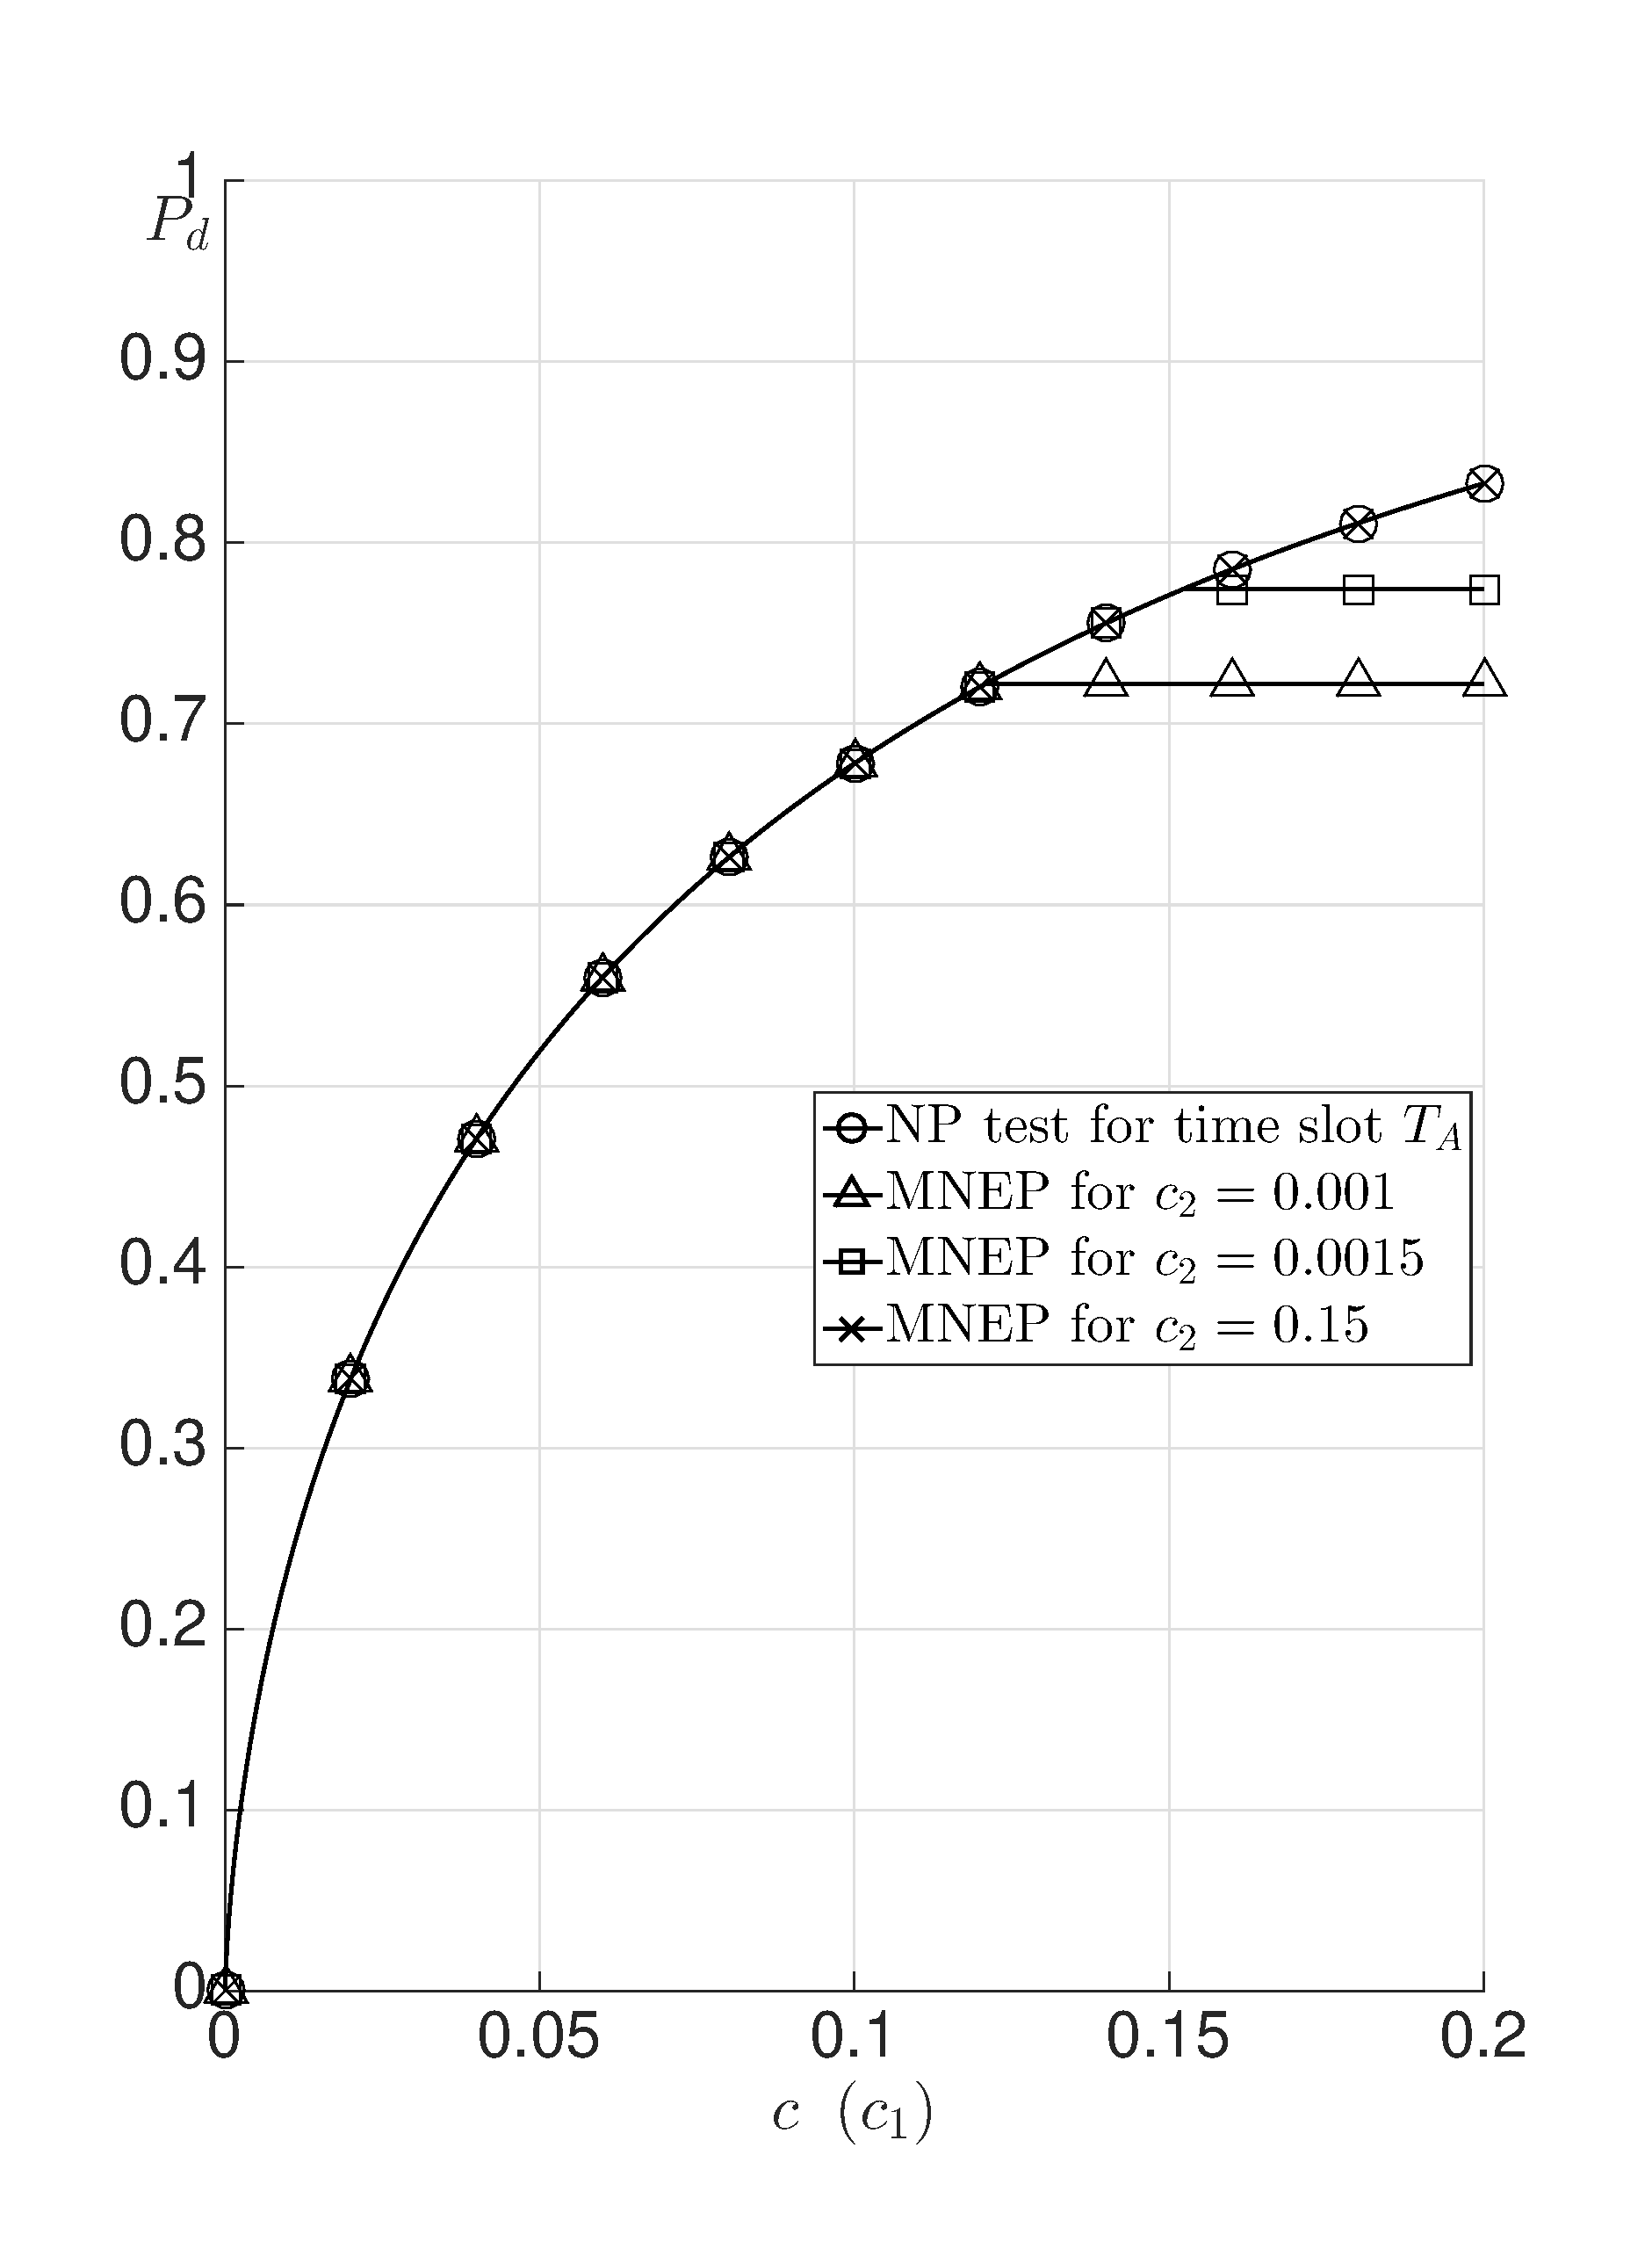
\includegraphics[width = 14cm]{5/SIa.eps}
  \caption{A comparison between the NP test and the MENP test during time slot $T_A$.} 
  \label{pic:20150702a0}
\end{figure} 

During time slot $T_A$, only primary signal $s_A$ could be present in the channel. Under the MENP framework, $P_{f_1}$ is the probability that the detector recognizes that the channel is free while $s_A$ is present. 
Hence under the MENP framework, we consider the relationship between $P_d$ and $c_1$. The performance of the MENP test is illustrated in Figure \ref{pic:20150702a0}.  

As we can observe, with $c_2$  fixed to $0.001$ (or $0.0015$), when $c_1$ is smaller than $0.12$ (or $0.15$) the performance of the MENP test and the NP test are the same; when $c_1$ is larger than $0.12$ (or $0.15$) the NP test has better performance. This is reasonable.  
For both MENP and NP tests with perfect side information, the decision rule can be written in form of
\begin{equation}
  y  \substack{\bar{H}_0 \\ \geq \\ < \\ H_0} V_\tau
\end{equation}
and the probability of detection is 
\begin{equation}
  P_d = F_0(V_\tau)\,.
\end{equation}
The above equation suggests $P_d$ is an increasing function with $V_\tau$. 
In the MENP test, $V_\tau$ is determined by $V_{\tau MENP}= \min (F_1^{-1}(c_1), F_2^{-1}(c_2))$; in the NP test with perfect side information, during time slot $T_A$, $V_\tau$ is determined by $V_{\tau NP A} = F_1^{-1}(c)$. When $c_1 \leq F_1(F_2^{-1}(c_2))$, i.e. $F_1^{-1}(c_1) \leq  F_2^{-1}(c_2)$, we have  $V_{\tau MENP} = F_1^{-1}(c_1)$. Since $V_{\tau NP A} = F_1^{-1}(c)$, when $c = c_1$, we have $V_{\tau MENP} = V_{\tau NPA}$, i.e.  $P_d(\delta_M) = P_d(\delta_{NP})$.    
When $c_1 > F_1(F_2^{-1}(c_2))$, i.e. $F_1^{-1}(c_1) > F_2^{-1}(c_2)$, we have  $V_{\tau MENP} = F_2^{-1}(c_2) < F_1^{-1}(c_1)$. Since $V_{\tau NP A} = F_1^{-1}(c)$, when $c = c_1$, we have 
$V_{\tau MENP} < V_{\tau NP}$, i.e.  $P_d(\delta_M) < P_d(\delta_{NP})$.
Hence for the MENP test, with $c_2$ fixed, when $c_1$ is smaller than $F_1( F_2^{-1}(c_2) ) $, $P_d(\delta_M) = P_d(\delta_{NP})$; when $c_1$ is larger than $ F_1( F_2^{-1}(c_2))$, $P_d(\delta_M) < P_d(\delta_{NP})$. 
However for the situation when  $c_2$ is fixed to $0.15$, for $c_1 \in [0, 0.2]$, $c_1 <  F_1(F_2^{-1}(c_2))$ is always holds. Hence for the situation when $c_2$ is fixed to $0.15$ and $c_1 = c \leq 0.2$, the performance of the MENP test and the NP test are the same. This is seen in Figure \ref{pic:20150702a0}. 

Next we consider the performance of the NP test and the MENP test during time slot $T_B$.
The performance of the NP and the MNEP tests are shown in Figure \ref{pic:20150704a0}. During time slot $T_B$, only primary user $s_B$ could present in the channel. Under the MENP framework, $P_{f_2}$ is the probability that the detector recognizes the channel is free while $s_B$ is present. Hence under the MENP framework, we consider the relationship between $P_d$ and $c_2$.

\begin{figure}[!hbp]
  \centering
  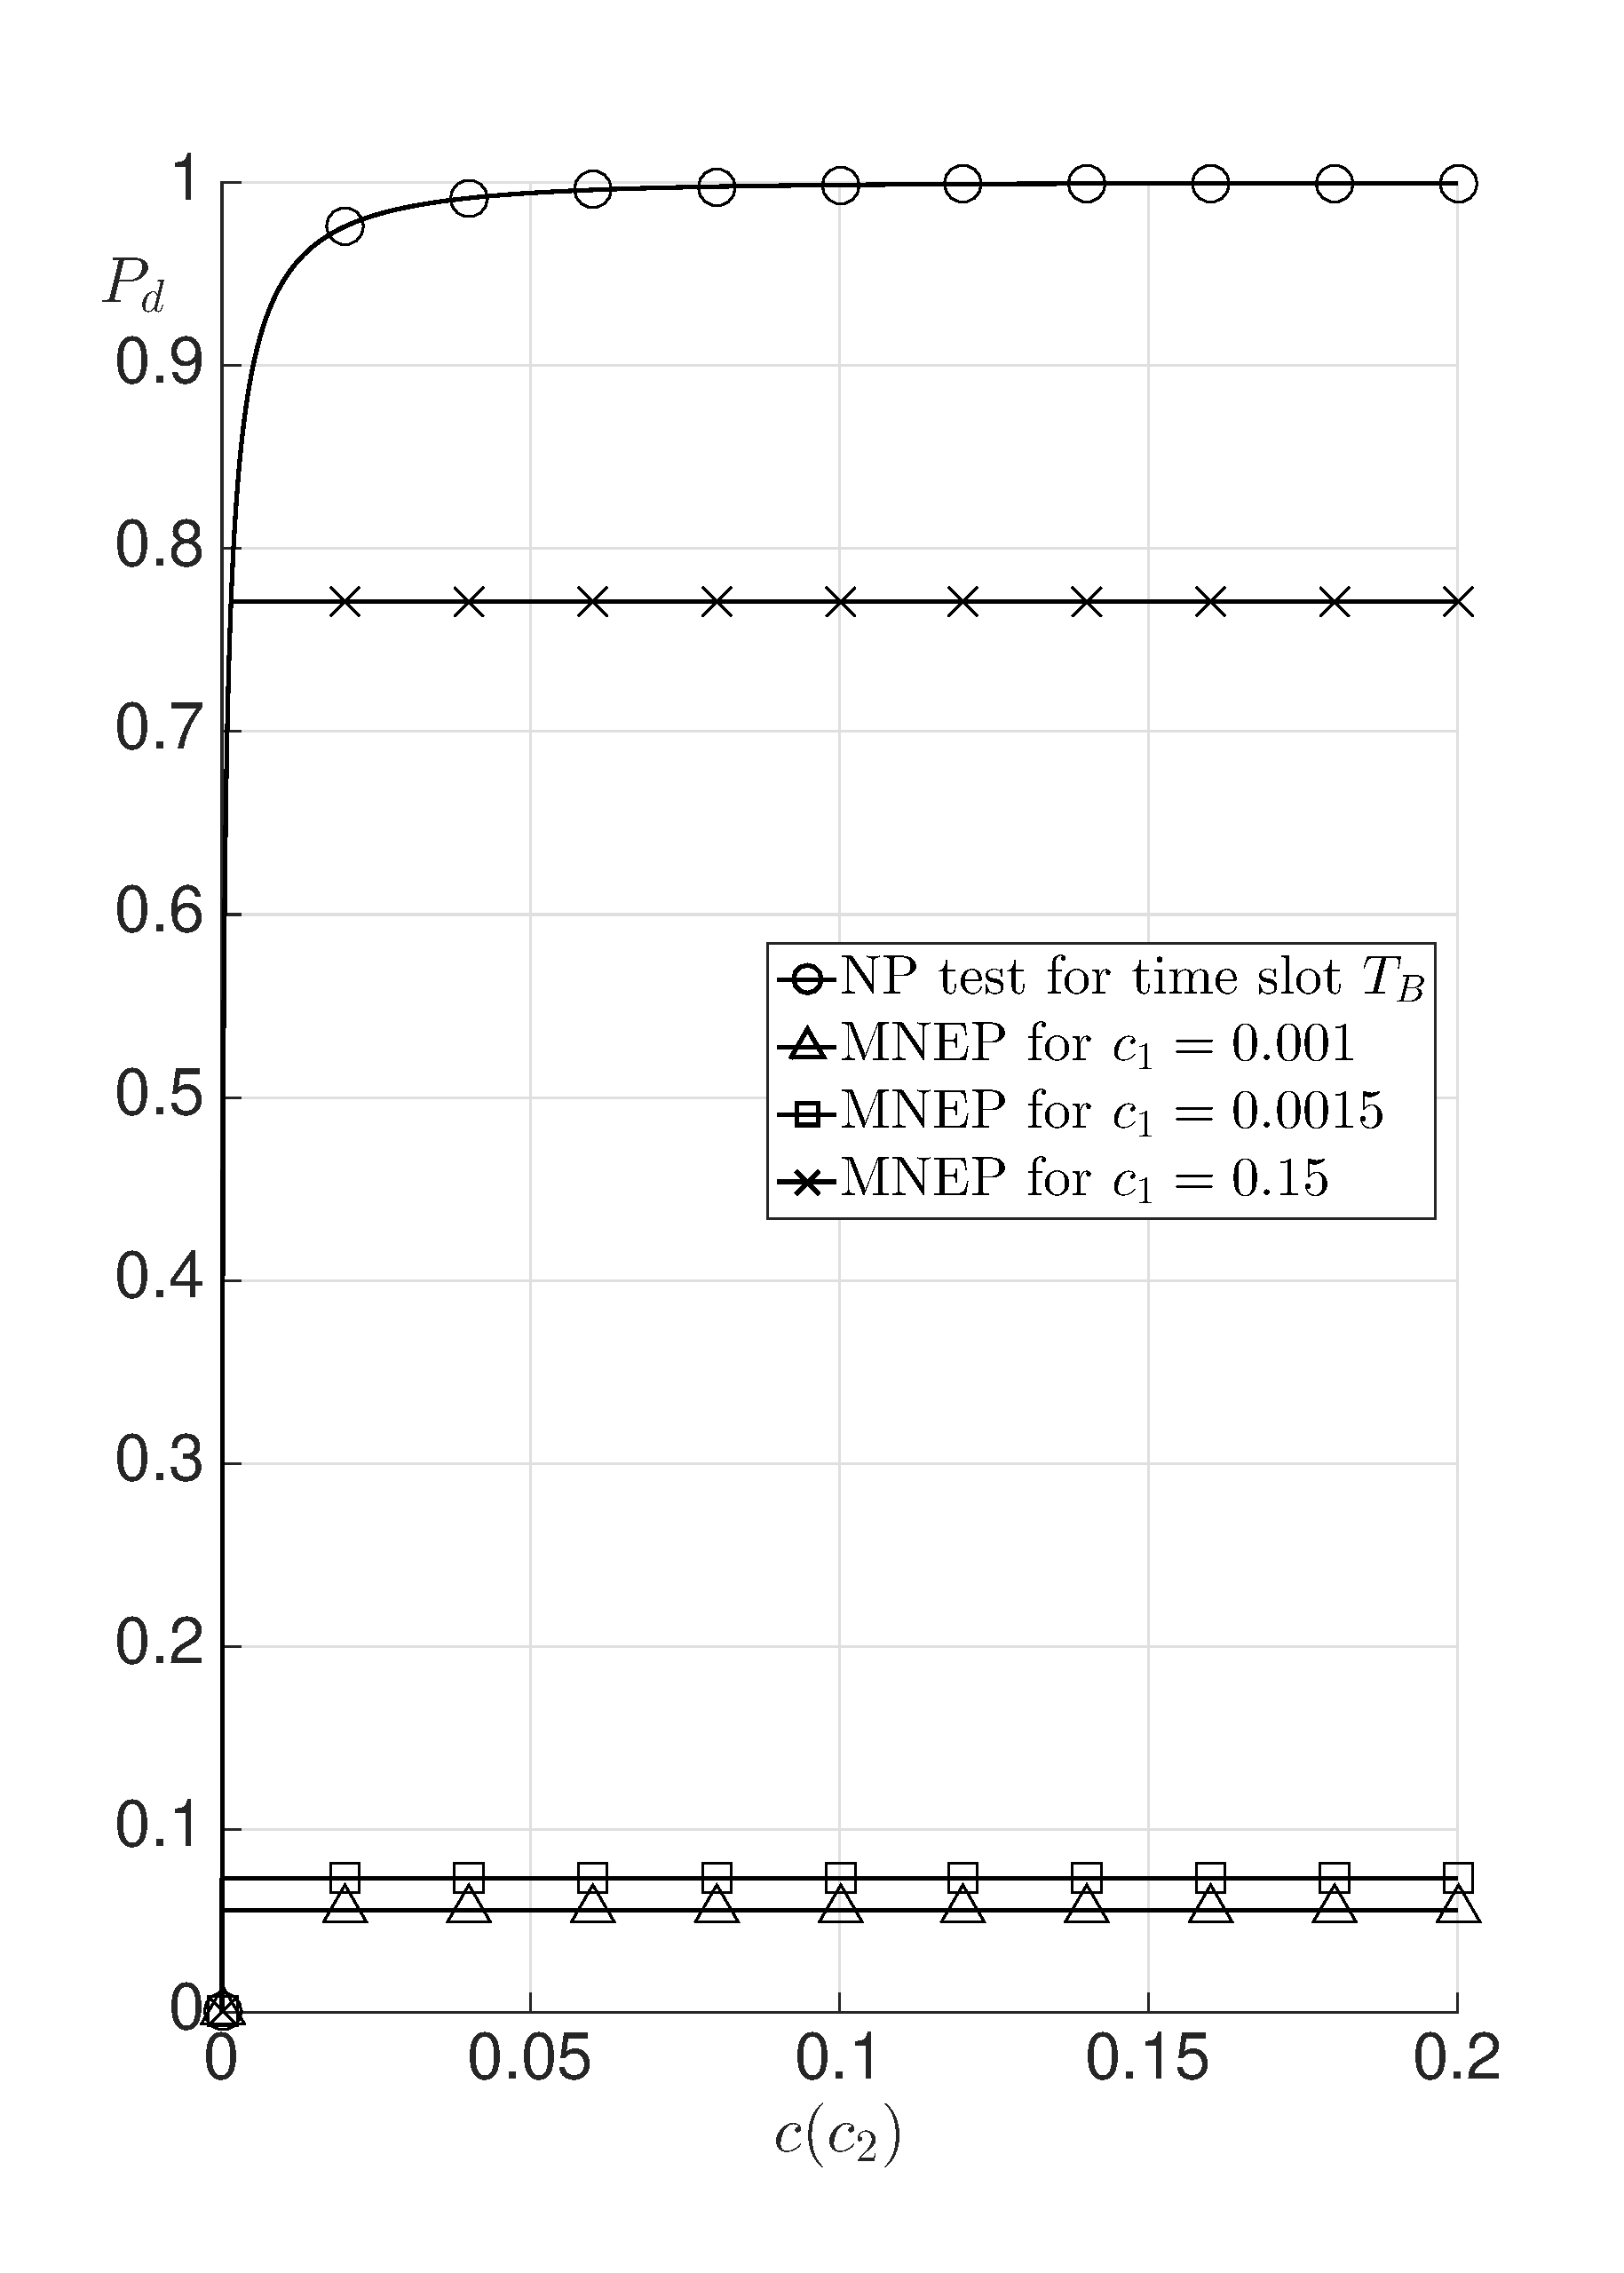
\includegraphics[width = 14cm]{5/SIb.eps}
  \caption{A comparison between the NP test and the MENP test during time slot $T_B$.} 
  \label{pic:20150704a0}
\end{figure} 

As we can observe, with $c_1$  fixed, when $c_2$ is small the performance of the MENP test and the NP test are the same; when $c_2$ becomes larger the NP test has better performance. This is reasonable. In the MENP test, $V_\tau$ is determined by $V_{\tau MENP}= \min (F_1^{-1}(c_1), F_2^{-1}(c_2))$; in the NP test with perfect side information, during time slot $T_B$, $V_\tau$ is determined by $V_{\tau NP B} = F_2^{-1}(c)$. When $c_2 \leq F_2(F_1^{-1}(c_1))$, i.e. $F_1^{-1}(c_1) \geq  F_2^{-1}(c_2)$, we have  $V_{\tau MENP} = F_2^{-1}(c_2)$. Since $V_{\tau NP B} = F_2^{-1}(c)$, when $c = c_2$, we have $V_{\tau MENP} = V_{\tau NP B}$, i.e. $P_d(\delta_M) = P_d(\delta_{NP})$.    
When $c_2 > F_1(F_2^{-1}(c_1))$, i.e. $F_1^{-1}(c_1) < F_2^{-1}(c_2)$, we have  $V_{\tau MENP} = F_1^{-1}(c_1) < F_2^{-1}(c_2)$. Since $V_{\tau NP B} = F_2^{-1}(c)$, when $c = c_2$, we have  $V_{\tau MENP} < V_{\tau NP B}$, i.e.  $P_d(\delta_M) < P_d(\delta_{NP})$.
Hence for the MENP test, with $c_1$ fixed, when $c_2$ is smaller than $ F_2( F_1^{-1}(c_1)) $, $P_d(\delta_M) = P_d(\delta_{NP})$; when $c_2$ is larger than $ F_2( F_1^{-1}(c_1)) $, $P_d(\delta_M) < P_d(\delta_{NP})$. 

From the above discussion, we can conclude that the NP test outperforms the MENP test when the detector has perfect side information. With $c_1$ ($c_2$) fixed, when $c_2$ ($c_1$) is small the performance of the  MENP test and the NP test are the same; when $c_2$ ($c_1$) becomes larger the NP test has better performance.  

